\documentclass[DIV=12]{scrartcl}
\usepackage{dsfont}
\usepackage{tikz}
\usepackage{caption}
\usepackage{fancyhdr}
\usepackage{amsmath}
\usepackage{amsthm}
\usepackage{enumerate}
\usepackage{enumitem}
\usepackage{amssymb}
\usepackage{amsfonts}
\usepackage{bbm}
\usepackage{graphicx}
\usepackage{hyperref}
\usepackage[ngerman]{babel}
\usepackage[OT1]{fontenc}
\usepackage{comfortaa}
\graphicspath{{img/}}
\usetikzlibrary{tikzmark}
\renewcommand{\sfdefault}{comfortaa}

\title{Einführung in die Theoretische Informatik}
\author{Felix Ichters\thanks{Universität Heidelberg}}
\date{Sommersemester 2023}

\begin{document}
\maketitle
\rule{\textwidth}{0.4pt}
\begin{abstract}
\begin{flushright}
    \textit{Begleitmaterial zur Vorlesung 'Einführung in die Theoretische Informatik'.}
\end{flushright}    
\end{abstract}
\par\bigskip
\begin{center}
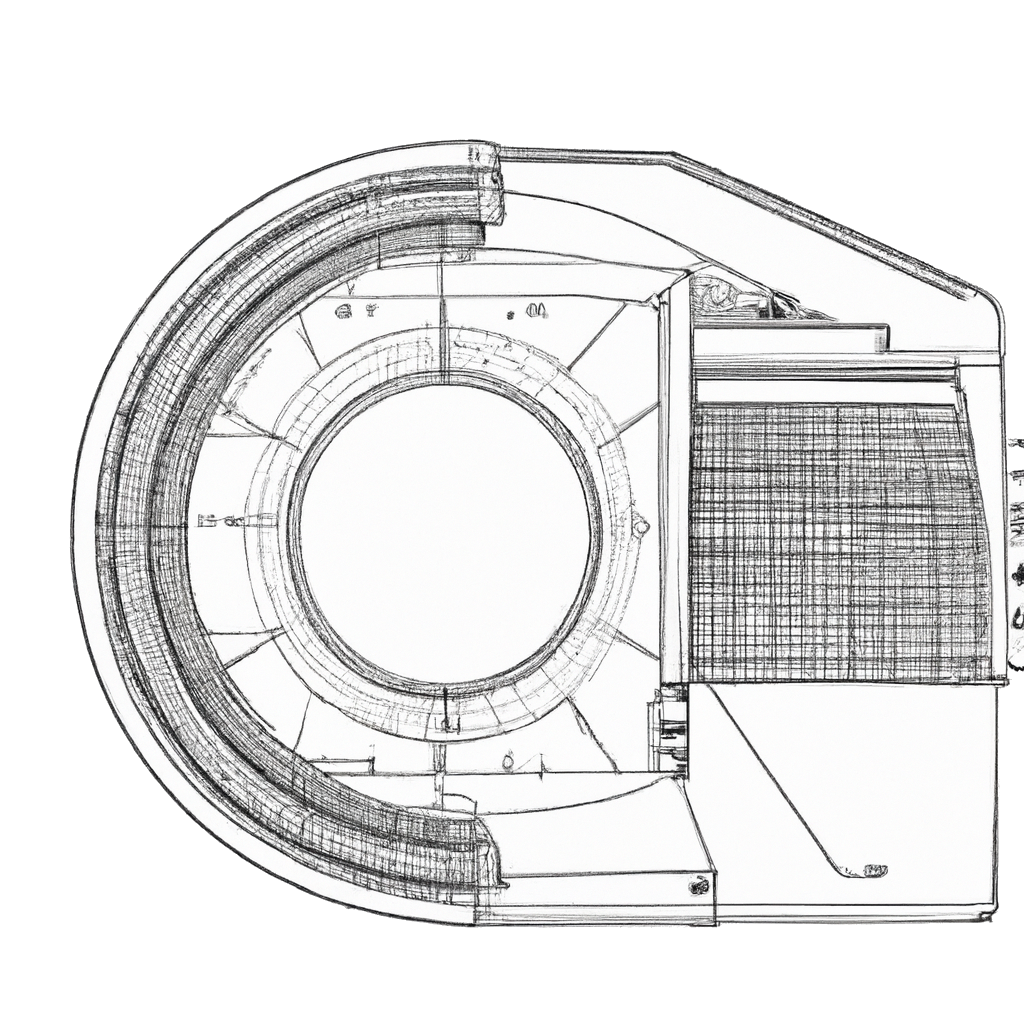
\includegraphics[width=0.5\textwidth]{dall2.png}    
\end{center}

\newpage
\tableofcontents
\newpage
\part{Definitionen}
\rule{\textwidth}{0.4pt}
\newpage
\section*{Notationen}
\rule{\textwidth}{0.4pt}\bigskip
\begin{itemize}
    \item Für \(n\in\mathbb{N}_0\), sei \([n]=\{1,\dots,n\}\) und \([n]_0=\{0,1,\dots,n\}\).
    \item Für eine Menge A und \(n\in\mathbb{N}\) ist \(A^n=\{(a_1,\dots,a_n):a_1,\dots,a_n\in A\}\).
    \item Für \(n\in\mathbb{N}\) ist eine n-äre partielle Funktion \(\varphi:A^n\rightsquigarrow B\) eine Funktion
    mit \(dom(\varphi)\subseteq A^n\) und \(Im(\varphi)\subseteq B\).
    Für \(a_1,\dots,a_n\in A\) bedeutet \(\varphi(a_1,\dots,a_n)\downarrow\), dass \(a_1,\dots,a_n\in dom(\varphi)\) gilt und 
    \(\varphi(a_1,\dots,a_n)\uparrow\) beduetet, dass \((a_1,\dots,a_n)\notin dom(\varphi)\).
    Die partielle Funktion \(\varphi\) ist total, wenn \(dom(\varphi)=A^n\) gilt.
    \item Eine lineare Ordnung auch totale Ordnung, auf einer Menge A ist eine Relation \(\leq\subseteq A^2\), so dass 
    die folgenden Eigenschaften erfüllt sind
        \subitem \(a\leq a\) \(\forall a\in A\) (Reflexivität)
        \subitem \(a\leq b\wedge b\leq a\Rightarrow a=b\) \(\forall a,b\in A\) (Antisymmetrie)
        \subitem \(a\leq b,b\leq c\Rightarrow a\leq c\) \(\forall a,b,c\in A\) (Transitivität)
        \subitem \(a\leq b\vee b\leq a\) \(\forall a,b\in A\) (Totalität)
\end{itemize}
\pagestyle{fancy}
\fancyhead{}
\section{Grundlagen}
\rule{\textwidth}{0.4pt}
\newpage
\subsection{Alphabet}
    Ein Alphabet ist eine nichtleere Menge \(\Sigma\),die Elemente heißen Symbole.
\subsection{Wörter}
    Ein Wort über einem Alphabet \(\Sigma\) ist eine endliche Folge von Symbolen aus \(\Sigma\).\\
    Für \(i\in[|w|]\) bezeichnet \(w(i)\) das i-te Element von w und für Symbole \(a_1,\dots,a_n\in \Sigma\)
    bezeichnet \(a_1,a_2,\dots,a_n\) das Wort w der Länge n mit \(w(i)=a_i\) \(\forall i\in [n]\).
\subsection{Sprache}
    Eine Sprache ist eine Menge von Wörtern über einem gemeinsamen Alphabet \(\Sigma\).
\subsection{\(\Sigma^*\)}
    Die Menge aller Wörter über \(\Sigma\) wird mit \(\Sigma^*\) bezeichnet.\\
    Für \(n\in\mathbb{N}_0\) setzen wir
    \[\Sigma^{\leq n}:=\{w\in\Sigma^*:|w|\leq n\}\]
    \[\Sigma^{=n}:=\{w\in\Sigma^*:|w|=n\}\]
    \[\Sigma^{\geq n}:=\{w\in\Sigma^*:|w|\geq n\}\]
    \[\Sigma^{+}:=\Sigma^{\geq 1}\]
\subsection{Verkettung}
    Für Wörter \(w_1,w_2\) ist die Verkettung \(w_1w_2\) ist definiert durch 
    \[w_1w_2:=w_1(1)\dots w_1(|w_1|)w_2(1)\dots w_2(|w_2|).\]
    Für Sprachen \(L_1,L_2\) sei \(L_1L_2\) definiert durch 
    \[L_1L_2:=\{w_1w_2:w_1\in L_1, w_2\in L_2\}\]
\subsection{Präfix, Infix, Suffix}
    Seien u,v Wörter 
    \begin{itemize}
        \item u ist Präfix von v, kurz \(u\sqsubseteq v\), falls es ein Wort w gibt, sodass uw=v 
        \item u ist Infix von v, falls es Wörter \(w_1,w_2\) gibt, sodass \(v=w_1uw_2\)
        \item u ist Suffix von v, falls es ein Wort w gibt, sodass v=wu
    \end{itemize}
\subsection{Homomorphismus}
    Für Sprachen \(L,M\) heißt eine Funktion \(\varphi:L\to M\) 
    Homomorphismus von Sprachen, wenn gilt: \[\varphi(uv) = \varphi(u)\varphi(v)\]
\subsection{Längenlexikographische Ordnungen}
    Es gilt \(u \leq_{llex} v\) wenn eine der folgenden Bedingungen erfüllt ist:
    \begin{enumerate}
        \item \(|u|<|v|\)
        \item \(|u|=|v|\) und ist \(i\in[|u|]\) minimal mit \(u(i)\ne v(i)\), so gilt \(u(i)\leq v(i)\)
    \end{enumerate}
\subsection{bin(i)}
\(bin(i)\) ist die Funktion für das in Längenlexikopraphischer Reihnfolge \(i+1\)-te Binärwort.\\
\(1bin(i)\) beschreibt die Binärdarstellung von \(i+1\).
\section{Turingmaschienen} 
\rule{\textwidth}{0.4pt}
\newpage
\subsection{Turingmaschiene}
    Eine k-Band Turingmaschiene ist ein Tupel \[M=(Q,\Sigma,\Gamma,\Delta,s,F)\]
    \begin{itemize}
        \item \(Q\) ist die endliche Zustandsmenge
        \item \(\Sigma\) ist das Eingabealphabet
        \item \(\Gamma\) das Bandalphabet mit \(\Sigma\subseteq\Gamma\) und \(\square\in\Gamma\backslash\Sigma\)
        \item \(\Delta\subseteq Q\times\Gamma^k\times Q\times\Gamma^k\times {\{L,S,R\}}^k\) die Übergangsrelation
        \item \(s\in Q\) der Startzustand
        \item \(F\subseteq Q\) die Menge der akzeptierten Zustände
    \end{itemize}
    Die Elemente von \(\Delta\) heißen Instruktionen, eine Instruktion sieht wie folgt aus:
    \[(q,a_1,\dots,a_k,q',a'_1,\dots,a'_k,B_1,\dots,B_k)\]
    \textit{Eine TM ist eine DTM, wenn es \(\forall b\in Q\times\Gamma^k\) höchstens eine Instruktion \(i\in \Delta\) mit Bedingungsteil b gibt}
\subsection{Konfiguration}
    Eine Konfiguration einer k-TM ist ein Tupel 
    \[C=(q,w_1,\dots,w_k,p_1,\dots,p_k)\in Q \times (\Gamma^*)^k \times \mathbb{N}^k\]
    Die Startkonfiguration zur Eingabe \((u_1,\dots,u_n)\in(\Sigma^*)^n\) mit \(n\in\mathbb{N}\), ist die Konfiguration
    \[start(u_1,\dots,u_n)=(s,u_1\square u_2\square\dots\square u_n,\square,\dots,\square,1,\dots,1)\]
    \textit{Die Stoppkonfiguartion ist die Konfiguration zu der es keine Nachfolgekonfiguration gibt}
\subsection{Nachfolgekonfiguration}
    Für Konfigurationen \(C=(q,w_1,\dots,w_k,p_1,\dots,p_k)\) und \(C'=(q',w'_1,\dots,w'_k,p'_1,\dots,p'_k)\) einer k-TM, \\
    ist die Konfiguration \(C'\) \textbf{Nachfolgekonfiguration} von C, wenn es eine Instruktion 
    \[(q,w_1(p_1),\dots,w_k(p_k),q',a'_1,\dots,a'_k,B_1,\dots,B_k)\in\Delta\] 
    gibt sodass
    \[
    w_i = \begin{cases}
        \square a'_iw_i(2)\dots w_i(|w_i|) & \text{ falls } p_i=1 \text{ und } B_i=L\\
        w_i(1)\dots w_i(|w_i|-1)a'_i\square & \text{ falls } p_i=|w_i| \text{ und } B_i = R\\
        w_i(1)\dots w_i(p_1-1)a'_iw_i(p_i+1)\dots w_i(|w_i|) & \text{ sonst}
    \end{cases}    
    \]
    und 
    \[
    w_i = \begin{cases}
        1 & \text{ falls } p_i=1 \text{ und } B_i=L\\
        p_i-1 & \text{ falls } p_i \geq 2 \text{ und } B_i = L\\
        p_i & \text{ falls } B_i=S\\
        p_i+1 & \text{ falls } B_i=R
    \end{cases}    
    \]
    für alle \(i\in [k]\) gelten.
\subsection{Rechnung}
    \textit{Es bezeichne \(\to _M\) die Relation auf der Menge der Konfigurationen einer k-TM M, sodass \(C\to _M C'\) \\
    falls \(C,C'\) Konfigurationen von M sind wobei C' eine Nachfolgekonfiguration von C ist.} \par\bigskip
    Eine \textbf{endliche partielle Rechnung} ist eine endliche Folge \(C_1,\dots,C_n\) von Konfigurationen von 
    M mit \(C_i\to _M C_{i+1}\forall i\in[n-1]\).\\
    Eine \textbf{unendlich partielle Rechnung} ist eine unendliche Folge \(C_1,C_2,\dots\) von Konfigurationen von 
    M mit \(C_i\to _M C_{i+1}\forall i+1\in\mathbb{N}\).
    Eine Rechnung zur Eingabe \((w_1,\dots,w_n)\in(\Sigma^*)^n\) mit \(n\in \mathbb{N}\) ist ein 
    unendlich partielle Rechnung \(start_M(w_1,\dots,w_n)=C_1,C_2,\dots,C_m\).
    \par\bigskip
    \textit{Ist M eine k-DTM, so gilt es \(\forall n \in \mathbb{N}\) und \((w_1, \cdots, w_n) \in (\Sigma^*)^n\) genau eine Rechnung zur Eingabe \((w_1, \cdots, w_n)\).}
    Ist M eine k-DTM, so gilt es \(\forall n \in \mathbb{N}\) und \((w_1, \cdots, w_n) \in (\Sigma^*)^n\) genau eine Rechnung zur Eingabe \(w_1, \cdots, w_n)\).
\subsection{Total}
    Totale TMs, sind TMs die bei jeder Eingabe immer anhalten. Alle Rechnungen müssen endlich sein.
\subsection{Akzeptierte Sprache}
    \textit{Eine Stoppkonfiguration ist akzeptiert, wenn \(q\in F\).}\par\bigskip
    Die akzeptierte Sprache L(M) ist die Sprache über dem Alphabet \(\Sigma\), so dass \(\forall w\in\Sigma^*\) genau dann 
    \(w\in L(M)\) gilt, wenn es eine endliche Rechnung \(C_1,\dots,C_n\) zur Eingabe w gibt, bei der \(C_n\) eine 
    akzeptierte Stoppkonfiguartion ist.\par\bigskip
    \textit{Für nicht-deterministische Tms heißt das, dass es für die Wörter in der akzeptierten Sprache nur mind. eine in einer 
    akzeptierten Stoppkonfiguartion endende endliche Rechnungen zur Eingabe w geben muss.\\
    Für Wörter w die nicht in L(M) sind, sind alle Rechnung von M zur Eingabe am Ende nicht in einer akzeptierten Stoppkonfiguartion oder unendlich}
\subsection{Entscheidbar}
    Eine Sprache L ist genau dann entscheidbar, wenn es eine totale k-TM mit L(M) = L gibt.
\subsection{Rekursiv aufzählbar}
    Eine Sprache L ist genau dann rekursiv aufzählbar, wenn es eine k-TM mit akzeptierter Sprache L gibt.\par\bigskip
    \textit{Wir schreiben RE für die Klasse der rekursiv aufzählbaren Sprachen. Die Aufzählbarkeit leitet sih daraus ab, dass es für eine rekuriv aufzählbare Sprache L über einem Alühabet $\Sigma$ möglich ist effektive Verfahren anzugeben ,die die Wörter von L aufzählen, also dass eine endlich oder unendliche Aufzählung von $A = w_1, w_2, \cdots$ mit ${w_1, w_2, \cdots} = L$ existiert.
    \begin{itemize}
        \item Jede entscheidbare Sprache ist rekuriv aufzählbar
        \item Alle endlichen Sprachen sind entscheidbar 
        \item Eine Sprache L über einem Alphabet $\Sigma$ist genau dann entscheidbar, wenn $L$ und $L^c :=(\Sigma^*)/L$ rekursiv aufzähbar sind.
    \end{itemize}
    }
\subsection{Ausgabe} 
    Die Ausgabe \(out_M(C)\) bei Konfiguration C ist das Präfix \(w\sqsubseteq w_1(p_1)\dots w_1(|w_1|)\) max. Länge mit 
    \(w\in (\Gamma\backslash\{\square\})^*\).\par\bigskip
    \textit{Also das längst mögliche Wort, dass auf Band 1 rechts vom Lesekopf steht und nicht \(\square\) enthält.}
\subsection{Berechnete Funktion}
    Sei M eine k-DTM. Die von M berechnete n-äre partielle Funktion \(\varphi_M\) ist die partielle Funktion:
    \[\varphi_M:(\Sigma^*)^n\rightsquigarrow(\Gamma\backslash\{\square\})^*\]
    sodass folgendes gilt:
    \begin{enumerate}
        \item Ist die Rechnung zur Eingabe \(w_1,\dots,w_n\) die endliche Rechnung \(C_1,\dots,C_m\) so gilt\\ 
        \(\varphi_M(w_1,\dots,w_n)=out_M(C_m)\)
        \item Ist die Rechnung zur Eingabe \(w_1,\dots,w_n\) unendlich, so gilt \(\varphi_M(w_1,\dots,w_n)\uparrow\)
    \end{enumerate}\bigskip
    \textit{Nur deterministische TMs können Funktionen berechnen.}
\subsection{Partiell Berechnbar}
    Für \(\Sigma,\Gamma\) und eine partielle Funktion \(U:\Sigma^*\rightsquigarrow\Gamma^*\) ist \(\varphi\) berechenbar, 
    wenn es ein \(k\in\mathbb{N}\) gibt und eine k-DTM M mit \(\varphi_M=\varphi\) gibt.\\
    Ist \(\varphi\) total und partiell berechenbar, so ist \(\varphi\) berechenbar.
\subsection{Charakteristische Funktion}
    Sei L eine Sprache über dem Alphabet \(\Sigma\).
    \begin{enumerate}
        \item Die charakteristische Funktion von L als Sprache über \(\Sigma\) ist die Funktion\\
        \(\mathbbm{1}_L:\Sigma^*\to\{0,1\}\) mit \(\mathbbm{1}_L(w)=1\) \(\forall w\in L\) und \(\mathbbm{1}_L(w)=0\) \(\forall w\in\Sigma^*\backslash L\).
        \item Die partiell charakteristische Funktion von L als Sprache über \(\Sigma\) ist die partielle Funktion\\
        \(\chi_L:\Sigma^*\rightsquigarrow\{1\}\) mit \(\chi_L(w)=1\) \(\forall w\in L\) und \(\chi_L(w)\uparrow\) \(\forall w\in\Sigma^*\backslash L\).
    \end{enumerate}
    \subsubsection*{Bemerkung}
        Sei L eine Sprache über einem Alphabet \(\Sigma\)
        \begin{itemize}
            \item L ist genau dann entscheidbar, wenn $\mathbbm{1}_L$ berechenbar ist.
            \item L ist genau dann rekursiv aufzähbar, wenn $x_L$ partiell berechenbar ist.
        \end{itemize}
\subsection{Normiet}
    Eine 1-DTM M heißt normiert, wenn Q={0,...,n} für ein \(n\in\mathbb{N}_0\), \(\Sigma=\{0,1\}\), \(\Gamma=\{\square,0,1\}\), \(\Delta=0\), \(F=\{s\}\).\par\bigskip
    \textit{
        Alle TMs mit Eingabealphabet {0,1} lassen sich mit folgenden Schritten in eine normierte TM mit gleicher erkannter Sprache und gleicher berechneten Funktion umwandeln.}
    \begin{itemize}
        \item Von nicht-Determinismus zu Determinismus
            \subitem Eine DTM kann die Rechnungen einer nicht-Deterministischen TM parallel im Sinne von abwechselnd schrittweise durchführen 
            um schließlich das Verhalten der simulierten TM zu imitieren.
            Das entspricht einer Breitensuche im Rechnungsbaum.
        \item Von mehreren Bändern zu einem Band
            \subitem Intuitiv können k Bänder auf einem Band simuliert werden, indem die Felder des einen Bandes in k-Teilfelder unterteilt werden, 
            die jeweils die gleichen Bandalphabetbuchstaben wie zuvor als Beschriftung zulassen und es zudem erlauben zu notieren, dass der simulierte Kopf des simulierten Bandes dort steht.  
        \item Von beliebigem Bandalphabet zu \(\{\square,0,1\}\)
        \subitem Andere Bandalphabete können bei einem Alphabet Wechsel zum Bandalphabet \(\{\square,0,1\}\) simuliert werden, 
        indem mehrere nebeneinander liegende Felder verwendet werden um ein Symbol des vorigen Bandalphabets durch ein Binärwort zu beschreiben .
        Die TM liest stets nur ein Feld, es wird daher also nötig sein die Zustandsmenge so zu erweitern, dass angrenzende Felder im Zustand gespeichert werden können.
    \end{itemize}
\subsection{Code}
    Wir betrachten die Funktion code mit geeigneter Definitionsmenge und Zielmenge \(\{0,1\}\).
    \begin{itemize}
        \item Codieren der Bewegungsrichtung
            \subitem \(code(L)=10\)
            \subitem \(code(S)=00\)
            \subitem \(code(R)=01\)
        \item Codieren der einzelnen Instruktionen
            \subitem \(I=(q,a,q',a',B)\)
            \subitem \(code(I)=0^{|bin(q)|}1bin(q)a0^{|bin(q')|}1bin(q')a'code(B)\)
        \item Codieren des Instruktinssatzes 
            \subitem \(code(\Delta)=code_1(\Delta)\dots code_{|\Delta|}(\Delta)\)
        \item Codieren der normierten TM 
            \subitem \(code(M)=0^{|bin(n)|}1bin(n)code(\Delta)\)    
    \end{itemize}
    \textit{Jede normierte TM hat einen Code und zwei verschiedene niemals den gleichen. Die Sprache der TMs ist entscheidbar.}   
\subsection{Standardaufzählung}
    \textit{Sei \(\hat{w}_0,\hat{w}_1,\dots\) die Aufzählung aller Codes normierter TMs in längenlexikopraphischer Ordnung.}\bigskip
    Für \(e\in\mathbb{N}\) sei \(\mathcal{M}_e\) die durch \(\hat{w}_e\) codierte TM und für \(n\in\mathbb{N}\) sei \(\Phi_e^n:\mathbb{N}_0^n\to\mathbb{N}_0\)
    die von \(\mathcal{M}_e\) berechnete n-äre partielle Funktion.\\
    Für \(n\in\mathbb{N}\) heißt die Folge \((\Phi_e^n)_e\in\mathbb{N}\) Standardaufzählung der n-ären partiell berechenbaren Funktion.\\
    Für \(n\in\mathbb{N}\) und eine partiell berechenbare n-äre partielle Funktion \(\varphi:\mathbb{N}_0^n\to\mathbb{N}_0\) heißt jede Zahl 
    \(e\in\mathbb{N}_0\) mit \(\Phi_e^n=\varphi\) Index von \(\varphi\).\par\bigskip
    \textit{Ergibt sich n aus dem Kontext so schreiben wir auch \(\Phi_e\) statt \(\Phi_e^n\)}\par\bigskip
    \textit{Für $n \in \mathbb{N}$ und eine partielle berechnbare n-äre partielle Funktion $\Phi : \mathbb{N}_0^n \rightarrow \mathbb{N}_0$ gibt es unendlich viele Indizes von $\varphi$.}
\subsection{U}
    Es bezeichne \(\mathcal{U}\) die normierte TM, bei Eingabe \((e,x_1,\dots,x_n)\in\mathbb{N}_0^{n+1}\) wobei \(n\in\mathbb{N}\) die normierte TM \(\mathcal{M}_e\)
    bei Eingabe \(x_1,\dots,x_n\) simuliert und falls diese terminiert die Asugabe der Simulation ausgibt.
\subsection{Universell}
    Eine DTM \(\mathcal{U}\) heßt universell, wenn es für alle \(n\in\mathbb{N}\) und alle partiell berechenbaren Funktionen \(\varphi:\mathbb{N}_0^n\rightsquigarrow\mathbb{N}_0\) 
    ein \(e\in\mathbb{N}_0\) gibt, sodass \(\mathcal{U}(e,x_1,\dots,x_n)=\varphi(x_1,\dots,x_n)\) für alle \(x_1,\dots,x_n\in\mathbb{N}_0\) gilt.
\subsection{s m n-Theorem}
    Für alle \(m,n\in\mathbb{N}\) existiert eine berechenbare Funktion \(s_n^m:\mathbb{N}_0^{m+1}\to\mathbb{N}_0\) mit 
    \[\Phi_e^{m+n}(x_1,\dots,x_m,y_1,\dots,y_n)=\Phi^n_{s_n^m(e,x_1,\dots,x_m)}(y_1,\dots,y_n)\]
    für alle \(e,x_1,\dots,x_m,y_1,\dots,y_n\in\mathbb{N}_0\).\par\bigskip
    \begin{proof}
        Fixiere $m \in \mathbb{N}$. Betrachte die DTM S , die bei Eingabe $(e, x_1, \cdots, x_m) \in \mathbb{N}_0^{m+1}$ wie folgt verfährt??.
\begin{itemize}
  \item Zunächst bestimmt S den Code von $\mathcal{M}_e$ 
  \item der Code von $\mathcal{M_e}$wird dann in einen Code einer normierten TM $\mathcal{M}$ umgewandet, die zunächst $x_1\Box\cdots\Box x_m\Box$ neben die Eingabe schreibt, dan den Kopf auf das erste Feld des beschriebenen Bandteilsbewegt und dann wie $\mathcal{M_e}$ arbeitet.
  \item Es wird bestimmt an welcher Stelle der Standardaufzählung der Code von auftaucht und diese Stelle wird ausgegeben.
\end{itemize}
Sei $s_n^m$ die von S berechnete $(m+1)$-äre partielle Funktion. Dann ist $s_n^m$ eine Funktion wie gewünscht.
    \end{proof}
\subsection{Diagonales Halteproblem}
    Die Menge \(H_{diag}:=\{e\in\mathbb{N}_0:\Phi_e(e)\downarrow\}\) heißt diagonales Halteproblem.\\
    \textit{Das diagonale Halteproblem ist rekursiv aufzählbar, jedoch nicht entscheidbar.}
\subsection{m-Reduktion}
    Für eine Sprache \(A\) über einem Alphabet \(\Sigma\) und eine Sprache \(B\) über einem Alphabet \(\Gamma\)
    ist \(A\) genau dann many-one-reduzierbar, auch m-reduzierbar, auf \(B\), kurs \(A\leq_m B\), wenn es eine berechenbare Funktion 
    \(f:\Sigma^*\to\Gamma^*\) gibt, so dass
    \[w\in A\Leftrightarrow f(w)\in B\]
    für alle \(w\in\Sigma^*\) gilt.\\
    \textit{gelten \(A\leq_m B\) und \(B\leq_m A\), so sind A und B m-äquibalent, kurz \(A=_m B\).}
\subsection{Postsches Korrespondenzproblem}
    Für ein Alphabet \(\Sigma\) sei eine Instanz des Postschen Korrespondenzproblem über \(\Sigma\)
    eine endliche Teilmenge \(I\subseteq(\Sigma^+)^2\) Eine Lösung für eine solche Instanz ist eine 
    endliche Folge \((u_1,v_1),\dots,(u_n,v_n)\) von Paaren in I mit \(n\geq1\), so dass 
    \[u_1\dots u_n=v_1\dots v_n\]
    Gibt es eine Lösung für eine Instanz des Postschen Korrespondenzproblems, so heißt diese Instanz lösbar.\\
    Das Postsche Korrespondenzproblem über einem Alphabet \(\Sigma\), kurz \(PCP_\Sigma\), ist die Menge 
    aller lösbarer Instanzen des Postschen Korrespondenzproblems über \(\Sigma\).\par\bigskip
    Für ein Alphabet \(\Sigma\) sei eine Instanz des modifizierten Postschen Korrespondenzproblems über \(\Sigma\)
    ein Paar \((p,I)\), wobei \(I\subseteq(\Sigma^+)^2\) eine endliche Teilmenge und \(p\in I\) ein Paar von Wörtern ist.\\
    Eine Lösung für ein solche Instanz ist eine endliche Folge \((u_1,v_1),\dots,(u_n,v_n)\) von Paaren in I, so dass 
    \[p=(u_1,v_1)\text{ und }u_1\dots u_n=v_1\dots v_n\]
    Gibt es ein Lösung für eine Instanz des modifizierten Postschen Korrespondenzproblems, so heißt diese Instanz lösbar.\\
    Das modifizierte Postsche Korrespondenzproblem über einem Alphabet \(\Sigma\), kurz \(MPCP_\Sigma\) ist die Menge aller 
    lösbarer Instanzen des modifizierten Postschen Korrespondenzproblems über \(\Sigma\).
\subsection{Fixpunkt}
    Ein Fixpunkt einer berechenbaren Funktion \(f:\mathbb{N}_0\to \mathbb{N}_0\) ist ein \(e\in\mathbb{N}_0\) mit 
    \(\Phi_{f(e)}=\Phi_e\).
\subsection{Rekursionstheorem}
    Für alle partiell berechenbaren Funktion \(\varphi:\mathbb{N}_0^2\rightsquigarrow\mathbb{N}_0\) gibt es ein 
    \(e\in\mathbb{N}_0\) mit \(\Phi_e(x)=\varphi(e,x)\forall x\in\mathbb{N}_0\).
\subsection{Indexmenge}
    Eine Teilmenge \(I\subseteq\mathbb{N}_0\) heißt Indexmenge, wenn \(e\in I\Leftrightarrow e'\in I\)
    für alle \(e,e'\in\mathbb{N}_0\) mit \(\Phi_e=\Phi_{e'}\) gilt.
\section{Automaten}
\rule{\textwidth}{0.4pt}
\newpage
\subsection{Endlicher Automat}
    Ein endlicher Automat, EA, ist ein Tupel \(A=(Q,\Sigma,\Delta,s,F)\).
    \begin{itemize}
        \item Q ist eine endliche Menge, die Zustandsmenge 
        \item \(\Sigma\) das Eingabealphabet
        \item \(\Delta\subseteq Q\times\Sigma\times Q \) die Übergangsrelation, so dass es 
        für alle \(q\in Q\) und \(a\in\Sigma\) ein \(q'\in Q\) mit \((q,a,q')\)
        \item \(s\in Q\) der Startzustand 
        \item \(F\subseteq Q\) die Menge der akzeptierenden Zustände
    \end{itemize}
    \textit{Der endliche Automat A ist ein deterministischer endlicher Automat, kurz DEA, wenn es
    \(\forall(q,a)\in Q\times\Sigma\) genau ein q' gibt mit \((q,a,q')\in\Delta\).
    Im Sinne der obigen Betrachtung entspricht ein EA \(A=(Q,\Sigma,\Delta,s,F)\) der 1-TM
    \(M_A=(Q,\Sigma,\Sigma\cup\{\square\},\{(q,a,q',a,R):(q,a,q')\in\Delta\},s,F)\).} 
\subsection{Übergangsfunktion eines EA}
    Die Übergangsfunktion eines EA A ist die Funktion \(\delta _A^*(q,\lambda)=\{q\}\) und
    \[\delta_A^*(q,aw)=\bigcup\limits_{q'\in\delta_A(q,a)}\delta_A^*(q',w)\] 
    \(\forall q\in Q,a\in\Sigma, w\in\Sigma^*\)\\
    Für \(Q_0\subseteq Q\) und \(w\in\Sigma^*\) schreiben wir \(\delta_A^*(Q_0,w)\) statt 
    \(\bigcup\limits_{q\in Q_0}\delta_A^*(q,w)\).\par\bigskip
    \textit{Sei A = (Q, $\Sigma$, $\Delta$, s, F) ein EA
    \begin{itemize}
        \item [(i)] $\forall$ q $\in$ Q und a$\in \Sigma$ gilt $\delta_{A}^{*}$(q,a) = $\delta_{A}$(q, a).
        \item [(ii)] Ist A ein DEA, q $\in$ Q, a $\in \Sigma$ und w $\in \Sigma^{*}$, und $\lvert \delta_{A}^{*}(q,w) \rvert$ = 1??.
        \item[(iii)] Seien u,v $\in \Sigma^{*}$ $\forall$ q $\in$ Q gilt $\delta_{A}^{*}$(q, uv) = $\delta_{A}^{*}(\delta_{A}^{*}(Q_{0}, u), v)$.
    \end{itemize}}
\subsection{Übergangsfunktion eines DEA}
    Sei A ein DEA. Auch die Funktion \(\delta_{det,A}:Q\times\Sigma\to Q\) mit \(\delta_a(q,a)=\{\delta_{drt,A}(q,a)\}\)
    \(\forall q\in Q\) und \(a\in \Sigma\) wird Übergangsfunktion von A genannt.
    Analoges gilt für \(\delta_{det,A}^*\) und \(\delta_A^*\).\\
    Für \(Q_0\subseteq Q\) und \(w\in\Sigma^*\) schreiben wir auch \(\delta_{det,A}^*(Q_0,w)\).\par\bigskip
    \textit{Sei Q eine endliche Menge, $\Sigma$ ein Alphabet, s$\in$ Q, und F$\subseteq$ Q. 
    \begin{itemize}
        \item [(i)] $\forall$ Funktionen $\delta$ : Q $\times \Sigma \rightarrow 2^{Q}$ gibt es genau einen EA A = (Q, $\Sigma$, $\Delta$, s, F) mit $\delta_{A}$ = $\delta$.
        \item [(ii)] $\forall$ Funktionen $\delta$ : Q $\times \Sigma \rightarrow$ Q gibt es genau einen $\delta_{det, A}$ = $\delta$. 
    \end{itemize}}
\subsection{akzeptierte Sprache}
    Sei A ein EA. Die Sprache \(L(A):=\{w\in\Sigma^*:\delta_A^*(s,w)\cap F\neq\varnothing\}\) ist die akzeptierte Sprache von A. 
\subsection{Regulär}
    Eine Sprache L heißt regulär, wenn es einen EA A mit L(A)=L gibt.\\
    Wir schreiben REG für die Klasse der regulären Sprachen.
    \subsubsection*{Beispiel}
    \textit{Zu jedem Zeitpunkt während der Verbindung der Eingabe durch einen endlichen Automaten höngt der restliche Bearbeitung immer nur vom gegewärtigen Zustand und dem noch einzulesenden Teil der Eingabe ab, nicht aber wie bei TM im allgemeinen von vergangenen Bandmanipulation. Interpretiert man die Eingabe als von einer äußeren Quelle kommend, so ist der  Zustand des Automaten also allein durch seinen Zustand gegeben und der nächste Zustand hängt nur vom Zugeführten Symbol ab. Daher bietet sich eine Darstellung eines EA durch ein Übergangsdiagramm oder eine sogenannte Übergangstabelle an.}\\
    Sei A := (\{$q_{0}$, $q_{1}$\}, \{0, 1\}, $\Delta$, $q_{0}$, \{$q_{1}$\}) mit $\Delta$ = \{($q_{0}$)\}
Übergangsdiagramm und übergangstabelle von sehen wie folgt aus:
\begin{center}
    \begin{tabular}{|c|c|c|}
        \hline
        Zustand/Symbol & 0 & 1 \\
        \hline
        $q_{0}$ & $q_{0}$ & $q_{1}$ \\
        \hline
        $q_{1}$, * & $q_{1}$ & $q_{0}$ \\
        \hline
    \end{tabular}            
\end{center}
\subsection{Übergangsdiagramm}
    Für jeden Zustand gibt es einen Kreis. Zustände in F bekommen einen Doppelkreis. Für \((q,a,q')\in\Delta\) für wir 
    einen Pfeil von dem Kreis von q zu dem Kreis von q' mit der Beschriftung a.\\
    Zustätzlich gibt es einen Pfeil (ohne Beschriftung) aus dem 'Nichts' zu dem Kreis des Startzustandes.
\subsection{Potenzautomat}
    Sei A ein EA. Der Potenzautomat von A ist der DEA \(P_a=(2^Q, \Sigma, \Delta',\{s\},\{P\subseteq Q:P\cap F\neq\varnothing\})\) mit
    \[\delta_{det,P_a}(Q_0,a)=\bigcup\limits_{q\in Q_0}\delta_A(q,a)\text{ }\forall Q_0\subseteq Q\text{ }\forall a\in\Sigma\]
    \subsubsection*{Satz}
        Eine Sprache L ist genau dann regulär, wenn es einen DEA A mit L(A) = L gibt.\par\bigskip
        \begin{proof}
            Sei A = (Q, $\Sigma$, $\Delta$, s, F) ein EA mit Potenzautomat $P_{A}$. Es genügt zu zeigen, dass L(A) = L($P_{A}$). Hierfür genügt es zu zeigen, dass:
\[\delta_{det,P}^{*} = \delta_{A}^{*}(s, w) \forall w \in \Sigma^{*} (*)\]
Denn damit folgt
\[w \in  L (P_{A}) \Leftrightarrow \delta_{P_{A}}^{*}(\{s\}, w) \cap \{P\subseteq Q : P\cap F \neq \varnothing \} \neq \varnothing \] 
\[\Leftrightarrow \delta_{det, P_{A}}^{*}(\{s\}, w) \cap F \neq \varnothing \]
\[\underset{\text{(*)}}{\Leftrightarrow } \delta_{A}^{*}(\{s\}, w) \cap F \neq \varnothing \]
\[\Leftrightarrow w \in L(A)\] Wir zeigen (*) mittels vollständiger Induktion über $\lvert$w$\rvert$. Es gilt $\delta_{det, P_{A}}^{*}$(\{s\}, $\lambda$) = $\delta_{A}^{*}$(s, $\lambda$). Sei w $\in \Sigma^{+}$ mit $\delta_{det, A}^{*}$(\{s\}, v) = $\delta_{A}^{*}$(s, v) $\forall$ v $\in \Sigma^{\leq \lvert w \rvert - 1}$. Nun zeigen wir (*) Sei va := w mit a $\in \Sigma$ und $\lvert$v$\rvert$ = $\lvert$w$\rvert$ - 1.
\[\delta_{det, P_{A}}^{*} (\{s\}, w) \underset{\text{Bem 4.5}}{=} \delta_{det, P_{A}}^{*} (\delta_{det, P_{A}}^{*}(\{s\}, v), a)\]
\[\underset{\text{Ind. hyp}}{=} \delta_{det, P_{A}}^{*}(\delta_{det, P_{A}}^{*}(\{s\}, v), a)\]
\[ = \bigcup \limits_{q \in \delta_{det, A}^{*}}\delta_{A}(q, a)\]
\[ = \delta_{A}^{*}(\delta_{A}^{*}(s, v), a)\]
\[ = \delta_{A}^{*}(s, va)\]
\[ = \delta_{A}^{*}(s, w)\]
        \end{proof}
\section{Reguläre Sprachen}
\rule{\textwidth}{0.4pt}
\textit{Wir verschieben den Fokus von endlichen Automaten auf die Klasse der von diesen erkannten Sprachen.
Dabei spielen endl. Automaten weiterhin eine wichtige Rolle.
Wegen 4.7 beschränken wir uns auf deterministische endliche Automaten.\\
Sei A DEA. Die Menge der zulässigen Eingaben \(\Sigma^*\) ist unendlich groß, 
die Menge der Zustände Q is aber endlich. Zwangsläufig wir A also das Einlesen verschiedener 
Eingaben im gleichen Zustand abschließen (und somit gleich behandeln). Dies führt zum Begriff
der A-Äquivalenz.}
\newpage
\subsection{Äquivalenzrelation}
    Sei A eine Menge. Eine Äquivalenzrelation auf A ist eine Relation \(\sim\subseteq A²\), so dass
    die folgenden Eigenschaften erfüllt sind.
    \begin{enumerate}
        \item \(a\sim a\) \(\forall a\in A\) (Reflexivität)
        \item \(a\sim b\Rightarrow b\sim a\) \(\forall a,b \in A\) (Symmetrie)
        \item \(a\sim b, b\sim c\Rightarrow a\sim c\) \(\forall a,b,c\in A\) (Transitivität)
    \end{enumerate}
    Die Äquivalenzklasse eines Elements \(a\in A\) bezüglich \(\sim\) ist die Menge 
    \([a]_\sim:=\{a'\in A:a'\sim a\}\). Der Index von \(\sim\) isr die Kardinalität
    der Menge \(A/{\sim}:=\{[a]_\sim:a\in A\}\) falls diese endlich ist und unendlich andernfalls.
\subsection{A-Äquivalenz}
    Sei A ein DEA. mit erweiterter Übergangsfunktion \(\delta^*:Q\times\Sigma\to Q\).\\
    Die A-Äquivalenz ist die Relation \(\sim_A\) auf \(\Sigma^*\) mit 
    \[u\sim_A v\Leftrightarrow \delta^*(s,u)=\delta^*(s,v)\text{ }\forall u,v\in\Sigma^*\]\par\bigskip
    \textit{\begin{itemize}
        \item [(i)] Die A-Äquivalenz ist eine Äquivalenzrelation.
        \item [(ii)] Der Index von $\sim_{A}$ ist höchstens $|Q|$.
        \item [(iii)] Es gilt $L(A) = \bigcup \limits_{w \in L(A)} [w]_{\sim A}$.
    \end{itemize}}
\subsection{Rechtskongurenz}
    Sei \(\Sigma\) ein Alphabet. Eine Rechtskongurenz auf \(\Sigma^*\) ist eine Äquivalenzrelation
    \(\sim\subseteq(\Sigma^*)^2\) mit \\
    \(u\sim v\Rightarrow uw\sim vw\) \(\forall u,v,w\in\Sigma^*\).\par\bigskip
    \subsubsection*{Proposition}
    Sei $A = (Q, \Sigma, \Delta, s, F)$ ein DEA. Die A-Äquivalenz $\sim_{A}$ ist eine Rechtskonqruenz auf $\Sigma^{*}$.

        \begin{proof}
          Seien $u, v, w \in \Sigma^{*}$ mit $u \sim_{A} v$. Dann gilt 
          \[\delta_{det, A}^{*}(s, uw) = \delta_{det,A}^{*}(\delta_{det,A}^{*}(s, u), w) = \delta_{det,A}^{*}(\delta_{det,A}^{*}(s,v), w)\]
          \[= \delta_{det,A}^{*}(s, vw).\]    
        \end{proof} Dann gilt $uw\sim_{A}vw.$
        $\Box $
        Zu jedem DEA A gibt es also eine dazugehärige Rechtskonguenz $\sim$ auf $\Sigma^{*}$ mit endlichem Index so dass L(A) die Vereinigung von Äquivalenzklasse von $\sim_{A}$ ist. Tatsächlich gilt auch die Umkehrung: Ist L die Vereinigung von Äquivalenzklasse einer Rechtskongruenz $\sim$ mit endlichem Index, so gibt es einen DEA A mit $L(A) = L$.
\subsection{}
    Sei \(\Sigma\) ein Alphabet und L Vereinigung von Äquivalenzklassen einer Rechtskongurenz \(\sim\)
    auf \(\Sigma^*\) mit endlichem Index. Es bezeichne 
    \[A_{\sim,L}:=(\Sigma^*/{\sim},\Sigma,\Delta,[\lambda]_\sim,\{[w]_\sim:w\in L\})\]
    den DEA mit \(\delta_{det,A_{\sim,L}}([w]_\sim,a)=[wa]_\sim\) \(\forall w\in\Sigma^*\) und \(a\in\Sigma\).
    \subsubsection*{Lemma}
    Sei $\Sigma$ ein Alphabet, L Vereinigung von Äquivalenzklassem einer Rechtskongruenz $\sim$ auf $\Sigma^{*}$ mit endlichem Index und sei $\delta^{*} : \Sigma^{*}_{/\sim} \times \Sigma^{*} \rightarrow \Sigma^{*}_{/\sim}$ die erweiterte Übergangsfunktion von $A_{\sim, L}$. Dann gilt $\delta^{*}([\lambda]_{\sim}, w) = [w]_{\sim} \forall w \in \Sigma^{*}$. 
\begin{proof}
  Wir verwenden vollständige Induktion über $|w|$. Es gilt $\delta^{*}([\lambda]_{\sim}, \lambda) = [\lambda_{\sim}]$. Sei nun $w \in \Sigma^{+}$ $\cdots$  
\end{proof}

\subsubsection*{Satz} Sei L die vereinigung von Äquivalenzklasse einer Rechtskongruenz $\sim$ mit endlichem Index Es gibt $L(A_{\sim, L}) = L$ 
\begin{proof}
  Sei $\Sigma$ das Alphabet, so dass $\sim$ eine Rechtskongruenz auf $\Sigma^{*}$ ist. Sei $\delta^{*} : \Sigma^{*}_{/\sim} \times \Sigma^{*} \rightarrow \Sigma^{*}_{/\sim}$ die erweiterte Übergangsfunktion von $A_{\sim, L}$ und sei $w \in \Sigma^{*}$. Es folgt 
  \[w \in L(A_{\sim, L}) \Leftrightarrow \delta^{*}([\lambda]_{\sim}, w) \in {[v]_{\sim} : v \in L}\]
  \[\Leftrightarrow [w]_{\sim} \in {[v]_{\sim} : v\in L}\]
  \[\Leftrightarrow \exists v \in L : [w]_{\sim} = [v]_{\sim}\]
  \[\Leftrightarrow \exists v \in L : w \sim v\]
  \[\Leftrightarrow w \in L\]
  $\cdots$    
\end{proof}

\subsubsection*{Korollar} Eine Sprache L ist genau dann regulär, wenn sie die Verienigung von Äquivalenzklasse einer Rechtskongruenz mit endlichem Index ist. 
\begin{proof}
  Folgt aus Bemerkung 5.3, Proposition 5.5 und Satz 5.8 $\Box$ 
\end{proof}
Betrachten man nur deterministische endliche Automaten ohne unerreichbare Zustände, so entsprechen diese bis auf Unbenutzung von Zuständen sogar den Rechtskongruenz mit endlichem Index zusammen mit Vereinigung von Äquivalenzklassn dieser.
\subsection{Erreichbar}
    Sei \(\Sigma\) ein Alphabet. Sei A ein EA mit erw. Übergangsfunktion \(\delta^*\). 
    Ein Zustand \(q\in Q\) heißt erreichbar in A wenn es ein Wort \\
    \(w\in\Sigma^*\) mit \(q\in\delta^*(s,w)\) gibt.
\subsection{Isomorph}
    Sei \(A_i\)für \(i\in\{1,2\}\) ein EA mit Übergangsfunktion \(\delta_i\).\\
    Die endlichen Automaten \(A_1\) und \(A_2\) sind Isomorph, kurz \(A\cong A_2 \), wenn es eine Projektion \\ \(f:Q_1\to Q_2\) gibt, so dass folgendes gilt:
    \begin{enumerate}
        \item \(f(s_1)=s_2\)
        \item \(\delta_2(f(q_1),a)=f(\delta_1(q_1,a))\) \(\forall q_1\in Q,a\in\Sigma\)
        \item \(f(F_1)=F_2\)
    \end{enumerate}
    \subsubsection*{Satz}
    \begin{itemize}
        \item [(i)] Ist $A$ eine DEA ohne unereichbare Zustände, so gilt $A \cong A_{\sim A, L(A)}$
        \item [(ii)] Ist L die Vereinuíngung von Äquivalenzklasse einer Rechtskongruenz $\sim$ mit endlichem Index, so gilt $(\sim, L) = (\sim_{A_{\sim, L}, L(A_{\sim, L})})$.
      \end{itemize}
    
      \begin{proof}
        \begin{itemize}
          \item [(i)] Sei $A = (Q, \Sigma, \Delta, s, F)$ eine DEA mit erweiterte Übergangsfunktion $\delta^* : Q \times \Sigma^* \to Q$ ohne unereichbare Zustände , $\sim := \sim_A$, $A' := A_{\sim, L(A)}$ und sei $\delta' : \Sigma^* / \sim \times \Sigma^* \to \Sigma/\sim$ die erweiterte Übergangsfunktion von $A'$. Sei $f : Q \to \Sigma^* / \sim$ die Bijektive mit $f(q) := \{ w \in \Sigma^* : \delta^*(s,w) = q\}$. Es gelte $f(s) = [\lambda]_{\sim}$ und $f(F) = \{[w]_{\sim} : w \in L(A)\}$. Es genügt somit zu zeigen , dass $\delta'(f(q), a) = f(\delta(q,a)) \forall q \in Q, a \in \Sigma$. Sei $q \in Q, a \in \Sigma^*$. Es genügt $w \in \delta' (f(q), a) \Leftrightarrow \delta^*(s,w) = \delta^*(q, a)$ zu zeigen. Sei $v \in \Sigma^*$ mit $\delta^*(s,v) = q$. Nun gilt $w \in \delta'(f(q), a) \leftrightarrow w \in \delta'([v]_{\sim}, a) \leftrightarrow w \sim va \leftrightarrow \delta^*(s,w) = \delta^*(s, va) \leftrightarrow \delta^*(s,w) = \delta^*(q,a)$  %füge hier bei dem letzetn pfeil noch "Bem 4.3 und 4.5" unter den pfeil hinzu"
          \item [(ii)] Sei $\Sigma$ ein Alphabet, $\sim$ eine Rechtskongruenz aud $\Sigma^*, L$ Vereinigung von Äquivalenzklassen von $\sim$, $A' := A_{\sim, L} = (\Sigma^*/\sim, \Sigma, A', [\lambda]_{\sim}, \uparrow)$, $\delta'^* : \Sigma^*/\sim \times \Sigma^* \to \Sigma^*/\sim$ die erweiterterte Übergangsfunktion von $A'$ $\{w \in \Sigma^* : w \in L \}$ und $\sim' := \sim_{A'}$. Nach Satz 5.8 gilt $L = L(A')$, es genügt also $\sim = \sim'$ zu zeigen. Sei $u, v \in \Sigma^*$. Aus lemma 5.7 folgt $u \sim v \leftrightarrow 
          [u]_{\sim} = [v]_{\sim} \leftrightarrow \delta'(...)$$\dots$
        \end{itemize}
      \end{proof}
\subsection{L-Äquivalenz}
    Sei L eine Sprache über einem Alphabet \(\Sigma\). Die L-Äquivalenz von L als Sprache ist die Relation \(\sim_L\) auf \(\Sigma^*\) mit 
    \[u\sim_L v\Leftrightarrow(uw\in L\Leftrightarrow vw\in L\text{ }\forall w\in\Sigma^*)\] 
    \subsubsection*{Bemerkung}
        Sei L eine Sprache über \(\Sigma\).
        \begin{enumerate}
            \item Die l-Äquivalenz ist eine Rechtskongurenz
            \item Es gilt \(L=\bigcup_{w\in L}[w]_{\sim L}\)
        \end{enumerate}
\subsection{Partition}
    Sei A eine Menge. Eine Partition von A ist eine Menge \(\mathcal{A}=\{A_1,\dots,A_n\}\) paarweise disjunkte nichtgeliche Teilmengen von A mit \(\bigcup_{i\in[w]}A_i=A\)
\subsection{Verfeinerung}
    Seien \(\mathcal{A}_1\) und \(\mathcal{A}_2\) Partitionen einer Menge A. Die Partition \(\mathcal{A}_2\) verfeinert \(\mathcal{A}_1\), wenn es \(\forall A_2\in\mathcal{A}_2\) ein \(A_i\in\mathcal{A}_1\), mit....
    \textit{
        Seien \(\mathcal{A}_1\) und \(\mathcal{A}_2\) Partitionen eine Menge A, so dass \(\mathcal{A}_2\) die Partition \(\mathcal{A}_1\) verfeinert.
        \begin{enumerate}
            \item \(\forall A'\in\mathcal{A}_1\), gibt es eine Teilmenge \(\mathcal{A}'_2\in\mathcal{A}_2\), die eine Partition von \(A'\) ist
            \item \dots
        \end{enumerate}}
    \subsubsection*{Proposition}
        \textit{Seien \(\Sigma\) ein Alphabet und L eine Sprache über \(\Sigma\) und \(\sim\) eine Rechtskongurenz auf \(\Sigma^*\) mit \(L=\bigcup_{w\in L}[w]_\sim\). Die Partition \(\Sigma^*\backslash\sim\) ist eine Verfeinerung der Partition \(\Sigma^*\backslash\sim_L\).}\par\bigskip
    \begin{proof}
        Seien \(u,v\in\Sigma^*\) mit \(u\sim v\). Es genügt zu zeigen, dass \(u\sim_Lv\).\\
        Sei \(w\in\Sigma*\). Es genügt \(uw\in L\Leftrightarrow vw\in L\) zu zeigen.\\
        Da \(\sim\) eine Rechtskongurenz ist folgt \(uw\sim vw\). Ist \(uw\in L\), so folgt aus \(L=\bigcup_{w'\in L}[w']_\sim\) auch \(vw\in L\) (analog folt auch \(vw\in L\Rightarrow uw\in L\)).\\
        \(\Rightarrow u\sim_Lv\)\\
    \end{proof}
        D.h. \(\sim_L\) ist die gröbste Partition, die L darstellen kann.
\subsection{Minimalautomat}
    Sei L eine reguläre Sprache über \(\Sigma\). Der Minimalautomat von L als Sprache über \(\Sigma\) ist der DEA \(A_{\sim_{L,L}}\)
    \subsubsection*{Satz}
        Sei L eine reguläre Sprache über \(\Sigma\) und sei M der Minimalautomat von L. Dann gilt:
        \begin{enumerate}
            \item \(L(M)=L\)
            \item ist A ein DEA mit Zustandsmenge \(Q_A\) und \(L(A)=L\), so gilt \(|Q_A|\geq|Q|\)
            \item ist A ein DEA mit \(|Q|\) Zuständen und \(L(A)=L\), so gitl \(A\cong M\) 
        \end{enumerate}
\section{Formale Grammatiken}
\fancyhead[R]{}
\fancyhead[C]{Formale Grammatiken}
\fancyhead[L]{Definitionen}
\paragraph*{Idee:} Konstruktion aller Wörter einer Sprache.
\paragraph*{Beispiel:} \(L=\{0^n\}_{n\in\mathbb{N}_0}\)\\
S Startsymbol\\
\(S\to X,S\to 0S\) Regel 
\(S\to 0S\to 00S\to 000S\to 000\)
\subsection{Grammatiken}
    Eine Grammatik ist ien Tupel \(G=(N,T,P,S)\). Dabei ist 
    \begin{itemize}
        \item N das Alphabet der Nichtterminalsymbole/Variablen 
        \item T das Alphabet der Terminalsymbole mit \(N\cup T=\varnothing \)
        \item \(P\subseteq((n\cup T)^*\backslash T^*)\times (N\cup T)^*\) eine endliche Menge von Regeln
        \item \(S\in\mathbb{N}\) das Startsymbol
    \end{itemize}
    EIne Satzform von G ist ein Wort \(s\in(N\cup T)^*\) und eine Terminalwort von G ist ein Wort \(t\in T^*\).
\subsection{Ableitung}
    Sei \(G=(N,T,P,S)\) eine Grammatik. Eine Satzform \(w'\) von G ist in einem Schritt aus einer Satzform w von G ableitbar, wenn es Satzformen u,v,x,y von G gibt, so dass \(w=xuy,u\to v\in P\) und \(w'=xvy\) gelten. Es bezeichne \(\to_G\) die Relation auf der Menge der Satzformen von G, sodass \(w\to_Gw'\) genau dann für Satzformen von G gilt, wenn w' aus w in einem Schritt ableitbar ist.\\
    Für Satzformen u,v von G ist eine Ableitung von v aus u eine Folge \(u=w_1,\dots,w_n=v\) mit \(w_i\to_Gw_{i+1}\) \(\forall i\in[n-1]\) und eine Ableitung von v in G ist eine Ableitung von v aus S in G. Für \(n\in\mathbb{N}\) schreiben wir \(u\to^n_Gv\) wenn es eine Ableitung von v aus u der Länge n gibt und wir schreiben \(u\to^*_Gv\) wenn eine Ableitung von v aus u in G existiert.
\subsection{Erzeugte Sprache}
    Sei \(G=N,T,P,S\) eine Grammatik. Die von G erzeugte Sprache \(L(G)\) ist die Menge aller Wörter \(w\in T^*\) für die es eine Ableitung von w in G gibt.
\paragraph*{Lemma} 
    Sei \(G=(N,T,P,S)\) eine Grammatik und seien u,v,x,y Satzformen von G und seien \(n,m\in\mathbb{N}\) mit \(u\to_G^nv\) und \(w\to_u^nxuy\).\\
    Dann gilt \(w\to_u^{m+n-1}xvy\).
\paragraph*{Beweis}
    Sei \(\alpha _1,\dots,\alpha_n\) ein Ableitung von xuy aus w und \(\beta_1,\dots,\beta_m\) eine Ableitung von v aus u. Dann ist\\ 
    \(\alpha_1,\dots,\alpha_{n-1},x\beta_1y,\dots,x\beta_my=xvy\)\\
    eine Ableitung von xvy aus w in G der Länge n+m-1.\par\bigskip
    Im folgenden beschäftigen wir uns mit dem Thema welche Sprache Grammatiken verschiedener Komplexitätsstufen erzeugen können.
\paragraph*{Satz}
    Eine Sprache ist genau dann rekuriv aufzählbar, wenn sie von einer Grammatik erzeugt wird.
\paragraph*{Beweisidee} Wird eine Sprache L von einer Grammatik erzeugt, so ist L die erkannte Sprache einer TM, die in geeigneter Weise Ableitungen von G erzeugt, prüft ob diese Ableitung dem Wort der Eingabe entspricht und gegebenfalss akzeptiert. Wenn eine Ableitung der Eingabe gefunden ist.\par\bigskip
Gegebn eine rekursiv aufzählbare Sprace L und eine TM, die L erkennt. So konstruieren wir ähnlich dem Postschen Korrespondenzproblems Regeln und Symobole, sodass wir die Arbeitsweise der TM modellieren können und entsprechend mit einem Terminalwort enden wenn dies von der TM erkannt wird.
\subsection{Rechtslinear}
    Eine Grammatik \(G=(N,T,P,S)\) ist rechtslinear, wenn alle Regeln von der Form 
    \[X\in uy \text{ oder } X\to u\]
    mit \(X,y\in\mathbb{N}\) und \(u\in T^*\) sind.\par\bigskip 
    Hier ist es sinnvoll endliche Automaten zu betrachten bei denen es nicht \(\forall\) Zustände q und Eingabesymbole a ein Tripel \((q,a,q')\) in der Übergangsrelation geben muss. Solche Automaten sind zwangsläufig nicht deterministisch.
\paragraph*{Satz}
Eine Sprache ist genu dann regulär, wenn sie von einer rechtslinearen Grammatik erzeugt wird.
\paragraph*{Beweisidee}
Zunächst überzeugt man sich davon, dass eine Sprache L genau dann von einer rechtlinearen Grammatik erzeugt wird, wenn sie von einer Grammatik \(G=(N,T,P,S)\) erzeugt wird bei der alle Regeln von der Form \(X\to ay\) oder \(X\to \lambda\)\\
mit \(x,y\in\mathbb{N}\) und \(a\in T\) sind. Eine Solche Grammatik wird als Grammatik in Simulationsform bezeichnet.\par\bigskip
Die Sprache L die von einer rechtslinearen Grammatik (in Simulationsform) gebildet wird von dem EA 
\[A=(N,T,\Delta,S,\{X\in N: X\to \lambda\in P\})\]
mit 
\[\Delta=\{(X,a,y)\in N\times T\times N:X\to ay\in P\}\]
erkannt.\\
Umgekehrt ist es einfach zu sehen, dass jede Reguläre Sprace von einer rechtslinearen Grammatik erzeugt wird.
\end{document}